\documentclass[letterpaper,10pt,conference]{ieeeconf}

\IEEEoverridecommandlockouts
\overrideIEEEmargins

\usepackage{amsmath,amssymb}
\usepackage{booktabs}
\usepackage{graphicx}
\usepackage{xcolor}
\usepackage{url}

\title{PIRoute: Online Policy Routing for Communication-Free Multi-Robot Navigation}
\author{Anonymous Authors}
\newcommand{\method}{PIRoute}
\newcommand{\fullsuccess}{full success}
\newcommand{\pendingdata}{\textcolor{red}{\bfseries DATA PENDING}}

\begin{document}
\maketitle
\thispagestyle{empty}
\pagestyle{empty}

\begin{abstract}
In shared spaces without communication, each robot must reach its goal from onboard observations while reacting to the other robots. A single policy must support both efficient goal progress and conservative collision avoidance, although the local interaction pattern changes over a rollout. We present \method, an online policy-routing framework for decentralized multi-robot navigation. The method reuses two pretrained actors, freezes them, and trains only a temporal router. The Interaction Actor was previously trained with privileged centralized supervision. At each routing instant, the router selects between their candidate actions using local LiDAR, motion state, observation history, and candidate-action disagreement. Its training signal combines a simulator-derived interaction-phase label with a same-state paired one-step reward comparison of the two frozen actors; neither signal is available at deployment. On the high-conflict multi-robot scenarios used in this study, a matched evaluation on the fixed high-conflict test set improves episode-level multi-agent full success from 24.61\% to 38.54\% and reduces robot-level collision from 31.72\% to 22.63\% relative to the Navigation Actor. The router incurs a 12.90-step increase on jointly successful episodes and selects the Interaction Actor on 70.57\% of routing frames.
\end{abstract}

\section{Introduction}
Multi-robot navigation in a shared workspace is coupled even when robots do not communicate. A robot changes the future observations of the others through its speed, heading, and waiting decisions. Rollouts alternate between ordinary goal progress and short periods of yielding, slowing, or conflict resolution. A controller therefore needs to identify the local interaction phase and return to goal-directed motion when that phase ends.

Many learning-based systems use one policy for both behaviors. The policy must then represent two different preferences: progress in ordinary states and conservative motion during dense interactions. Episode-level selection is also insufficient. Different robots can be in different interaction states at the same time, and one robot can enter and leave an interaction within a single episode. A distance rule based on other robots' positions can indicate when conditional control would help, but that information is unavailable to a decentralized robot at deployment.

We ask whether two pretrained policies with complementary behavior can be routed from local observations when training uses both interaction-phase and action-outcome supervision. \method{} freezes a Navigation Actor and an Interaction Actor, then learns a temporal router for each robot. During training, simulator robot positions provide a binary interaction-phase target. Isolated same-state one-step branches provide a paired reward difference between the candidate actions. At deployment, the privileged states and reward values are removed, as are communication and global conflict information. Separate temporal encoders predict the two targets. A fixed bounded fusion rule combines them, followed by hysteresis and a minimum hold time before one actor is selected.

\method{} formulates policy reuse as a per-robot routing problem under local-observation deployment constraints. Its training objective combines a privileged interaction-phase label with the relative one-step outcome of the two candidate actions, while neither target is available to the deployed router. We evaluate the resulting frozen-policy system in closed loop and report team success, robot-level collision, completion steps, and policy-selection frequency.

\section{Related Work}
\textbf{Decentralized multi-robot navigation.} Reciprocal velocity obstacles impose geometric collision-avoidance constraints, whereas CADRL learns a decentralized policy for non-communicating agents \cite{vanDenBerg2008,chen2017cadrl}. Later policies extend learned collision avoidance to denser crowds and pedestrian-rich settings \cite{long2018decentralized,everett2021collision}, and mapless navigation has also been transferred from simulation to physical robots \cite{tai2017virtual}. Recent work addresses complementary limitations, including certifiable safety and connectivity \cite{Cui_2022,Li_2022}, perception in narrow spaces and communication-restricted coordination \cite{Park_2023,Bramblett_2023}, and distributional, socially aware, or goal-conditioned navigation \cite{Lin_2024,Wang_2024,Feng_2025}. These systems generally optimize a single deployed policy. We instead retain two specialized policies and learn when each robot should use them from local observations.

Cooperative multi-agent reinforcement learning commonly uses centralized training with decentralized execution, including actor--critic, counterfactual, and monotonic value-factorization methods \cite{lowe2017maddpg,foerster2018coma,rashid2018qmix,gronauer2021marl}. Our setting instead freezes the policy experts and learns only a per-robot selector after expert training.

\textbf{Temporal policy selection.} Options formalize temporally extended policies and their termination conditions \cite{sutton1999options}. Option-Critic learns both components jointly, and deliberation costs discourage unnecessary switching \cite{bacon2017option,harb2018deliberation}. In navigation, APPLD, APPLI, and APPLR adapt planner parameters from demonstrations, interventions, or reinforcement learning \cite{xiao2020appld,wang2021appli,xu2021applr}. Other systems switch between classical and learned planners \cite{kastner2022allinone,dey2023trust}; Matsumoto et al. use a normalizing flow for this decision \cite{matsumoto2024flow}, while Kim et al. switch decentralized robots between artificial-potential-field and wall-following behaviors \cite{Kim_2025}. \method{} differs in three respects: selection is made separately for each robot, both learned policies remain frozen, and privileged supervision is removed at deployment. We evaluate the selector through closed-loop team outcomes rather than classification accuracy alone.

\textbf{Privileged supervision and closed-loop aggregation.} Asymmetric actor--critic methods give the critic privileged state while the deployed actor receives sensor observations \cite{pinto2018asymmetric}. Learning by Cheating instead transfers knowledge from a privileged teacher to a sensor policy \cite{chen2020cheating}. DAgger queries labels on learner-visited states, and SafeDAgger and EnsembleDAgger use intervention or uncertainty to regulate those queries \cite{ross2011dagger,zhang2017safedagger,menda2019ensemble}. Related safe-control methods constrain policies or actions through costs, shields, stability conditions, observation-based refinement, or trajectory optimization \cite{achiam2017cpo,alshiekh2018shielding,berkenkamp2017safe,dalal2018safe,Cui_2022,brunke2022safe}. Our privileged target labels the local interaction phase rather than supplying an expert action or value. Student-rollout states broaden the router's training distribution, but we do not attribute an independent performance gain to that aggregation step.

Off-policy continuous-control methods such as soft actor--critic and goal relabeling provide complementary training foundations for the frozen experts, but are not used as competing router designs here \cite{haarnoja2018sac,andrychowicz2017her}. Uncertainty estimation under dataset shift motivates keeping deployment-side switching evidence local and explicitly measurable \cite{ovadia2019trust}.

\section{Problem Formulation}
Consider $N$ robots. Each actor receives a 24-dimensional local observation
\begin{equation}
 o_t^i=[\ell_t^i,D_t^i,\theta_t^i,u_{t-1}^i]\in\mathbb{R}^{24},
\end{equation}
where $\ell_t^i\in\mathbb{R}^{20}$ is the 20-sector LiDAR encoding, $D_t^i$ and $\theta_t^i$ are goal distance and bearing error, and $u_{t-1}^i\in\mathbb{R}^{2}$ is the previous command. The deployed perception stack additionally reads the raw VLP-16 scan and ego odometry to construct router features. Robots do not exchange state, intent, or maps. Let $\pi_N$ and $\pi_I$ denote the Navigation Actor and Interaction Actor. Both receive the same deployable observation and produce candidate actions
\begin{equation}
 a_{N,t}^i=\pi_N(o_t^i),\qquad a_{I,t}^i=\pi_I(o_t^i),\qquad a\in\mathbb{R}^{2}.
\end{equation}
The actors emit tanh actions. Hard selection is formed in this raw action space. Before execution, the environment maps the selected linear component to its nonnegative velocity range. For the router comparison feature, that component is mapped from $[-1,1]$ to $[0,1]$ before $\Delta a_t^i=a_{I,t}^i-a_{N,t}^i$ is formed.
The router produces a binary state $z_t^i$ and executes a hard selection,
\begin{equation}
 a_t^i=(1-z_t^i)a_{N,t}^i+z_t^i a_{I,t}^i.
 \label{eq:hardroute}
\end{equation}
The actors are not updated during router training. A robot may therefore use a different actor from another robot at the same environment time.

During training only, the simulator provides robot centers $p_t^i$. Let $\mathcal{A}_t$ contain robots that are neither at the goal nor in collision immediately before the routing decision. For the nearest active robot, the interaction target is
\begin{equation}
 d_t^i=\min_{j\neq i,\,j\in\mathcal{A}_t}\|p_t^i-p_t^j\|_2,\qquad y_t^i=\mathbb{I}[d_t^i\leq 2.0\,\mathrm{m}].
 \label{eq:label}
\end{equation}
Equation~\eqref{eq:label} is a supervision proxy. It is not a deployable distance rule and does not imply that the Interaction Actor is optimal at every positive frame. If no other active robot exists, we set $d_t^i=+\infty$ and hence $y_t^i=0$. Robots that have reached their goals or have collided are removed from $\mathcal{A}_t$ and no longer contribute routing actions. The label can therefore include nearby but non-threatening robots. This proxy noise is part of the training protocol.

\section{PIRoute}
\subsection{Frozen Policy Library and Perception}
The Navigation Actor follows the TD3 actor--critic formulation~\cite{fujimoto2018td3}. Its actor was initialized from the preceding curriculum checkpoint; the critic was reinitialized before training on five-robot standard scenes with individual rewards and no neighborhood input. We selected the checkpoint by full success and use it for goal progress and static-obstacle handling. The Interaction Actor was initialized from the Navigation Actor and trained for 320,000 agent samples. During this second stage, the nearest-active-robot distance defined an interaction window ($\leq 2.0$\,m): the Interaction Actor was executed and updated inside the window, while the Navigation Actor controlled all other states. Its critic received a privileged 87-dimensional neighborhood observation, but the Interaction Actor retained the same 24-dimensional local observation used at deployment. Both actors were trained in the same simulator and frozen before router training; neighborhood information is unavailable at test time.

The LiDAR perception front end projects the VLP-16 scan into a local geometric representation. For each geometrically generated point-cloud candidate, it estimates a robot-shape probability in $[0,1]$ and a center offset. Simulator robot positions supervise both outputs during training. The deployment controller takes track centers from the geometric candidates and retains the robot-shape probability as a continuous feature; it does not use the learned center offset or make a hard robot/non-robot decision. The detector criterion was precision $\geq 0.70$, recall $\geq 0.90$, and overall false-positive rate (FPR) $\leq 0.10$, with static-obstacle FPR reported separately. Because the model did not satisfy all three conditions, \method{} treats its probability as soft evidence rather than as a reliable detection. A deterministic tracker smooths this probability and adds candidate age, relative velocity, closing speed, closest-point-of-approach, and time-to-collision features. The perception model and tracker are frozen before router training.

\subsection{Router Representation}
At each routing instant, the router forms a 76-dimensional local representation $q_t^i$ from local state, LiDAR candidate features, and short-term tracking. It also receives both candidate actions and their disagreement:
\begin{equation}
 \Delta a_t^i=a_{I,t}^i-a_{N,t}^i,\qquad x_t^i=[q_t^i,a_{N,t}^i,a_{I,t}^i,\Delta a_t^i]\in\mathbb{R}^{82}.
 \label{eq:routerinput}
\end{equation}
The action difference is a task-relevant cue rather than a value-function difference. It indicates when the two frozen roles recommend materially different controls.

\subsection{Temporal Estimation and Stable Switching}
The router encodes the latest $H=8$ routing frames with a GRU,
\begin{equation}
 \begin{aligned}
 \tilde h_{p,t}^i&=\mathrm{GRU}_{p}(x_{t-H+1:t}^i,\mathbf{0})_{\mathrm{last}},\\
 \tilde h_{r,t}^i&=\mathrm{GRU}_{r}(x_{t-H+1:t}^i,\mathbf{0})_{\mathrm{last}},\\
 \ell_t^i&=f_p(\tilde h_{p,t}^i),\quad p_t^i=\sigma(\ell_t^i),\\
 A_t^i&=f_r(\tilde h_{r,t}^i),\quad A_t^i\in[-1,1],\\
 g_t^i&=\sigma\!\left(\ell_t^i+\beta A_t^i\right).
 \end{aligned}
 \label{eq:gru}
\end{equation}
Here $p_t^i$ estimates the interaction-control phase, $A_t^i$ predicts a bounded transform of the paired one-step reward difference, and $g_t^i$ is the joint routing score. The two GRUs have independent parameters, so the smaller reward dataset does not alter the phase representation learned from all phase labels. The phase branch uses weighted binary cross-entropy against Eq.~\eqref{eq:label}, and the reward branch uses a scene-weighted Huber loss. We set $\beta=0.25$ before closed-loop evaluation. The router is evaluated every two environment steps. To suppress one-frame reversals, the binary state uses an entry threshold $\tau_{\rm on}=0.43$, an exit threshold $\tau_{\rm off}=0.33$, and a minimum hold of three routing evaluations:
\begin{equation}
 z_t^i=\begin{cases}
 1,&z_{t-1}^i=0\ \land\ g_t^i\geq\tau_{\rm on},\\
 0,&z_{t-1}^i=1\ \land\ g_t^i\leq\tau_{\rm off}\ \land\ c_t^i\geq 3,\\
 z_{t-1}^i,&\text{otherwise.}
 \end{cases}
 \label{eq:hysteresis}
\end{equation}
Here $z_t^i$ is initialized to zero. The counter $c_t^i$ counts router evaluations since entry into the Interaction Actor; it is reset on a mode change and incremented only while $z_t^i=1$. The selected actor recomputes an action from the new local state at every environment step. The mode is updated only at the routing stride. Only the selected action is applied to the simulator, although both actor forward passes are computed. Fig.~\ref{fig:overview} shows the information boundary.

\subsection{Training Protocol}
The perception front end is first trained with simulator-generated candidate supervision. We then freeze the perception model, deterministic tracker, $\pi_N$, and $\pi_I$. Navigation and student-rollout states provide the inputs in Eq.~\eqref{eq:routerinput} and the interaction labels in Eq.~\eqref{eq:label}. The phase branch uses all labeled states. The reward branch uses the smaller set of paired counterfactual samples that passed the state-alignment checks described below.

\subsection{Paired One-Step Reward Supervision}
For a stratified set of aligned anchors, two isolated one-step simulator branches execute $a_{N,t}^i$ and $a_{I,t}^i$ from the same state. Both branches use the same task reward. The fixed common reward uses $+100/-100$ for goal/collision transitions and weights $20$, $0.5$, $0.2$, $0.5$, and $0.03$ for progress, forward action, turning, obstacle, and stagnation terms. Cooperative and other auxiliary shaping terms are disabled. We define
\begin{equation}
 \begin{aligned}
 \Delta r_t^i&=R(s_t^i,a_{I,t}^i)-R(s_t^i,a_{N,t}^i),\\
 A_t^i&=\tanh\!\left(\frac{\operatorname{clip}(\Delta r_t^i,-s,s)}{s}\right),
 \end{aligned}
 \label{eq:rewardtarget}
\end{equation}
where $s$ is the training-only 95th percentile of the absolute per-anchor median reward difference. Under this sign convention, $\Delta r_t^i>0$ means that the Interaction Actor obtains the higher one-step reward, whereas $\Delta r_t^i<0$ favors the Navigation Actor. Terminal differences are retained as valid evidence and clipped by the bounded transform. The reward head predicts $A_t^i$. The phase and reward losses are optimized in separate branches with scene weighting for repeated counterfactual measurements. Simulator positions, branch rewards, and $\Delta r_t^i$ are training-only and never enter the deployed router. The reward-aware router is the only newly trained component; both actors and the perception/tracking stack remain frozen.

\subsection{Implementation Details}
Both frozen actors use the same 24-dimensional observation and a $24\!\to\!800\!\to\!600\!\to\!2$ MLP with ReLU hidden layers and tanh actions. The perception model is a three-layer CNN (16, 32, and 64 channels, $3\times3$ kernels, GroupNorm, ReLU, and $2\times2$ max-pooling in the first two blocks) followed by adaptive pooling and separate robot-shape and center-offset heads. Only its continuous robot-shape probability is passed to tracking. The deterministic tracker associates candidates within $0.65$ m, exponentially smooths the shape probability, retains up to two missed frames, and estimates motion from a five-frame history. Its four highest-priority tracks contribute $4\times11$ features, including raw and smoothed shape probabilities. Eight global summary features complete the 76-dimensional $q_t^i$ together with the 24-dimensional actor state. Tracks are sorted by detector confidence and motion risk, then zero-padded when fewer than four are present. The 82-dimensional router input is normalized using training-split statistics.

The router uses two independent single-layer 64-hidden-unit GRUs. Each is followed by a $64\!\to\!32\!\to\!1$ head; the reward head has a final tanh to enforce the bounded target. We optimize with Adam (learning rate $10^{-3}$, weight decay $10^{-4}$) using a fixed 40-epoch phase budget and 80-epoch reward budget. Best checkpoints are selected on disjoint validation data before any closed-loop test. Counterfactual reward supervision contains 548 training records from 356 unique anchors and 336 unique scenes, and 132 validation records from 65 unique scenes. Repeated measurements are scene-weighted. Router states are reset per episode and per robot. Histories shorter than eight routing frames are left-padded with zeros, and terminated robots are excluded from subsequent routing decisions. The router mode is evaluated every two environment steps. The selected actor recomputes its action every environment step; with a 0.2-s environment step, mode updates occur at 2.5 Hz. Thresholds are $0.43/0.33$, with fusion weight $\beta=0.25$ and a minimum hold of three routing evaluations.

Experiments use ROS Noetic with Gazebo 11.15.1. One action step advances 0.2 s, and Gazebo uses a fixed physics increment of 0.001 s. A robot succeeds when its center reaches within 0.30 m of its goal without collision; collision is recorded when the minimum LiDAR return falls below 0.35 m. Episodes end after 300 environment steps (60 s nominal simulation time). Evaluation seeds and checkpoint identities are recorded with the experimental protocol.

\begin{figure*}[t]
  \centering
  
\includegraphics[width=0.96\textwidth]{piroute_overleaf_fonts_fixed_20260908/generated/fig1_overview/Section 2-2 3.pdf}
  \caption{PIRoute information boundary. During deployment, each robot uses only local observation history, two frozen actor candidates, and a temporal router before executing one selected action. During simulation training, robot positions generate the interaction-phase target and isolated same-state branches provide paired one-step reward supervision; both signals are removed before deployment.}
  \label{fig:overview}
\end{figure*}

\section{Experimental Protocol}
\subsection{Research Questions and Comparisons}
Our primary question is whether reward-aware routing of the frozen policy pair improves closed-loop full success over the Navigation Actor in dense multi-robot interactions. Robot-level collision is the secondary safety metric; completion steps and Interaction Actor selection share quantify operating cost. We also compare against the Interaction Actor deployed alone, two rule-based selectors, and a parameter-matched Actor. A separately trained two-stage single Actor tests whether continued training of one policy can replace online routing. Results from the earlier proximity-only router and the privileged-distance selector are used only for diagnostic comparisons.

\subsection{Matched Evaluation}
The matched evaluation contains 256 fixed high-conflict test scenes and three environment repeats, giving 768 episodes per method. The reward-aware router was evaluated after the stored control results had been inspected, but it uses the same manifest, seeds, physics, checkpoints, and termination rules. The comparison is therefore matched rather than a new sealed test. The router evaluation and statistical analysis were specified before its queue was launched.

The primary metric is \emph{full success}: all five robots reach their goals within the termination condition without collision. We additionally report robot-level agent success and collision, episode timeout, raw termination steps, paired-success steps, Interaction Actor selection share, and switch counts. Full success is analyzed with scene-cluster paired bootstrap confidence intervals and a two-sided scene-level sign-flip test; repeated runs of the same scene are not treated as independent scenes. The privileged 2-m rule is diagnostic and non-deployable and is excluded from the matched evaluation.

\subsection{Implementation and Cost}
The actors and perception/tracking stack are frozen during router training. The control loop runs at 5 Hz, and the router updates its mode every two steps. We measured inference on an Intel Core i9-14900KF using one CPU thread, batch size 1, 200 warm-up iterations, and 2,000 timed iterations. With point-cloud candidates precomputed, perception/tracking features, two actor forwards, and router inference take 1.443 ms (p95 1.490 ms); a single Navigation Actor forward takes 0.037 ms. This benchmark measures inference rather than training and excludes point-cloud candidate extraction, ROS transport, sensor waiting, and command publication. \method{} therefore adds computation and requires both actor candidates at each routing instant.

\subsection{Scenarios and Splits}
All experiments use the Gazebo multi-robot navigation simulator with five differential-drive robots unless stated otherwise. The mixed-scene development set contains 120 fixed scenes, comprising 60 standard and 60 high-conflict scenes, with two environment repeats. A separate high-conflict development set contains 256 scenes: 8, 61, 80, and 107 have 0, 1, 2, and at least 3 reference-path conflict edges, respectively. These edges are used only to stratify scenes offline. They are not router or policy inputs. The matched evaluation uses a fixed 256-scene high-conflict test split with identical scenes and environment repeats for all methods. Training and validation scenes do not appear in this split. The qualitative trajectories were collected separately and do not contribute to any reported rate.

\subsection{Metrics and Statistical Analysis}
An episode is a full success only when every robot reaches its goal within the termination condition without collision. Agent success and collision are robot-level rates; unresolved denotes a robot that is neither successful nor colliding when an episode times out. We report collision over all robot outcomes rather than over episodes. Raw termination steps can be shortened by early collisions, so completion cost is also computed on matched scene--repeat pairs in which both methods achieve full success. Repeated runs are clustered by scene. Confidence intervals use a scene-cluster BCa paired bootstrap with 20,000 resamples, and $p$-values use a two-sided scene-level Monte Carlo sign-flip test with 100,000 draws. The analysis threshold is $\alpha=0.05$: the primary success claim requires both a positive confidence-interval lower bound and a sign-flip $p$-value below this threshold. Percentages are pooled descriptive rates; differences and intervals follow the paired clustered analysis.

\section{Results}
\subsection{Matched Evaluation}
All methods in Table~\ref{tab:main} use the same 256 high-conflict scenes and three environment repeats. The reward-aware runs completed every scene--repeat pair with consistent scenario ordering and terminal accounting.

\begin{table}[t]
\caption{Matched evaluation on the frozen high-conflict test set. Full success and timeout are episode-level rates, whereas agent success, collision, and unresolved are robot-level rates. Steps are environment steps; entries are percentages except Steps.}
\label{tab:main}
\centering
\scriptsize
\setlength{\tabcolsep}{2.5pt}
\begin{tabular}{lrrrrrr}
\toprule
Method & Full & Agent & Coll. & Unres. & Timeout & Steps\\
\midrule
Navigation Actor & 24.61 & 68.23 & 31.72 & 0.05 & 0.26 & 17.31\\
Interaction Actor only & 28.65 & 73.65 & 17.76 & 8.59 & 36.72 & 145.23\\
Min-LiDAR selector & 26.56 & 72.73 & 17.66 & 9.61 & 40.63 & 155.06\\
TTC/CPA selector & 27.47 & 69.56 & 30.31 & 0.13 & 0.65 & 20.60\\
Parameter-matched Actor & 25.52 & 68.57 & 31.41 & 0.03 & 0.13 & 16.89\\
Two-stage single Actor & \multicolumn{6}{c}{\pendingdata}\\
\textbf{Reward-aware router} & \textbf{38.54} & \textbf{77.29} & \textbf{22.63} & 0.08 & 0.39 & 32.11\\
\bottomrule
\end{tabular}
\end{table}

\begin{figure*}[t]
  \centering
  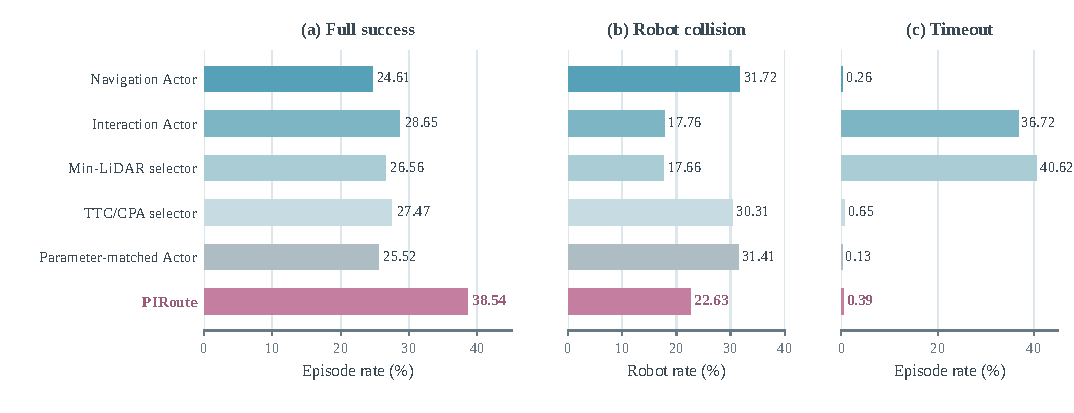
\includegraphics[width=\textwidth]{figures/fig2_method_comparison.pdf}
  \caption{Absolute performance of the complete deployable methods on the matched high-conflict test set. Bars show pooled descriptive rates over 768 episodes per method; collision is computed over 3,840 robot outcomes. The low collision rates of the Interaction Actor and Min-LiDAR selector coincide with frequent episode timeouts, whereas \method{} yields the highest full-success rate.}
  \label{fig:method_comparison}
\end{figure*}

\subsection{Main Results}
Relative to the Navigation Actor, \method{} raises full success by $13.93$ percentage points (scene-cluster BCa 95\% CI [$+9.51,+18.23$]; two-sided sign-flip $p=0.00001$) and lowers robot-level collision by $9.09$ percentage points (BCa 95\% CI [$-11.25,-7.03$]). Agent success increases by $9.06$ percentage points. Among 126 scene--repeat pairs in which both methods achieve full success, \method{} requires $12.90$ additional environment steps (BCa 95\% CI [$+10.06,+16.34$]). It selects the Interaction Actor on $70.57\%$ of routing frames and makes 7.41 switches per episode.

\begin{figure*}[t]
  \centering
  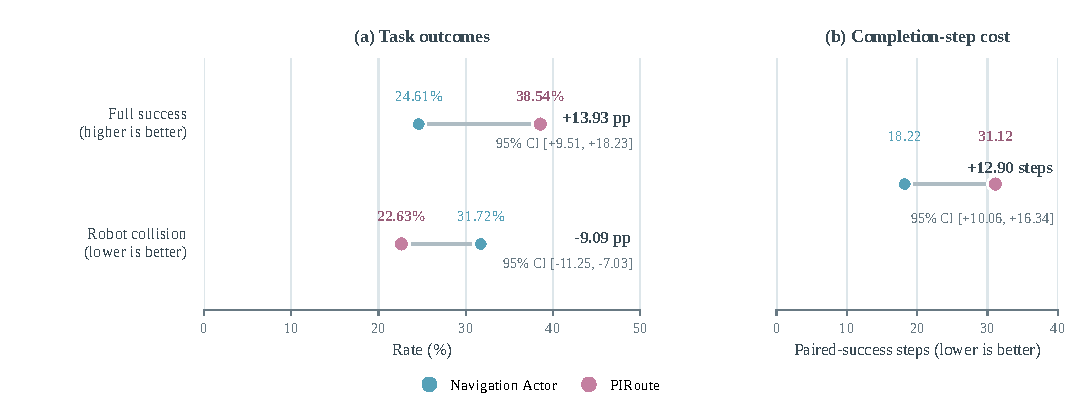
\includegraphics[width=\textwidth]{figures/fig3_paired_effects.pdf}
  \caption{Direct comparison between \method{} and the Navigation Actor. Connected endpoints show their pooled outcome rates and mean completion steps; labels report paired effect estimates with scene-cluster BCa 95\% confidence intervals. Completion steps use the 126 scene--repeat pairs in which both methods achieve full success.}
  \label{fig:paired_effects}
\end{figure*}

When deployed at every step, the Interaction Actor lowers robot-level collision to $17.76\%$, but its $36.72\%$ timeout rate limits full success to $28.65\%$. The Min-LiDAR selector shows a similar conservative failure mode, whereas the TTC/CPA selector and parameter-matched Actor remain close to the Navigation Actor in full success. The two-stage single Actor in Table~\ref{tab:main} is a separate control: one policy is first trained for standard navigation and then trained as the sole controller in high-conflict scenes. This comparison tests whether sequential specialization can recover the benefits of retaining two experts.

\subsection{Reward-Supervision Ablation}
To isolate the contribution of action-outcome supervision, we keep the same frozen dual-encoder checkpoint and set the reward-difference fusion weight from $0.25$ to zero. The phase encoder, actors, observations, thresholds, hysteresis, hold time, scenes, and environment repeats are unchanged.

\begin{table}[t]
\caption{Ablation of reward-difference evidence in the routing decision. Both variants use the same frozen actors, router checkpoint, scenes, and environment repeats. Entries follow the definitions in Table~\ref{tab:main}.}
\label{tab:reward_ablation}
\centering
\scriptsize
\setlength{\tabcolsep}{3pt}
\begin{tabular}{lrrrr}
\toprule
Variant & Full & Agent & Coll. & Steps\\
\midrule
Reward-aware routing & 38.54 & 77.29 & 22.63 & 32.11\\
Phase-supervision only & \multicolumn{4}{c}{\pendingdata}\\
\bottomrule
\end{tabular}
\end{table}

This comparison changes only whether the predicted reward difference contributes to the final routing score. It therefore separates the added action-outcome evidence from the temporal architecture and switching logic inherited by both variants.

\subsection{Qualitative Closed-Loop Evidence}
The qualitative capture contains four complete navigation--interaction--navigation cycles across 320 robot sequences. Fig.~\ref{fig:cycle} shows one such cycle: the robot enters Interaction Actor control during a local conflict and later returns to the Navigation Actor. These trajectories were recorded with the predecessor proximity-only router, which shares the temporal switching mechanism but not the reward-difference branch. The outcome-stratified, single-seed sample illustrates behavior rather than estimating cycle frequency or routing efficiency.

\begin{figure*}[t]
  \centering
  
\includegraphics[width=0.94\textwidth]{piroute_overleaf_fonts_fixed_20260908/generated/fig4_cycle/gate_cycle_example.pdf}
  \caption{Representative closed-loop cycle recorded with the predecessor proximity-only router. The robot executes the Navigation Actor, enters the Interaction Actor during a local conflict, and returns to Navigation Actor control before reaching its goal.}
  \label{fig:cycle}
\end{figure*}

\subsection{Generalization and External Switching Baseline}
Without additional training, the predecessor router improves full success by 3.13 percentage points with three robots and 1.56 percentage points with seven robots, although both exploratory confidence intervals cross zero. With seven robots, robot-level success increases by 9.54 percentage points (exploratory BCa 95\% CI [6.14, 12.72]) and collision decreases by 9.65 percentage points (95\% CI [$-12.83,-6.25$]); raw termination length increases by 17.42 steps. We also implement a normalizing-flow-inspired switch motivated by Matsumoto et al.~\cite{matsumoto2024flow}. On an independent five-robot split, it obtains 30.08\% full success, compared with 28.52\% for the Navigation Actor and 35.94\% for the proximity-only predecessor. Its 1.56-percentage-point difference from the Navigation Actor has an exploratory BCa 95\% CI of [$-4.30,+7.42$]. These experiments characterize the predecessor router and are analyzed separately from the matched evaluation of the reward-aware method.

\section{Limitations and Discussion}
The evidence is limited to a fixed policy library and matched high-conflict simulations. The distance-based phase label can mark nearby robots that do not require avoidance, which may contribute to the high Interaction Actor selection share and the additional steps on successful runs. Deployment also requires two actor forward passes at each routing instant.

The parameter-matched control follows the Navigation Actor training recipe, but its retained checkpoint precedes effective updates to the widened actor; later unfreezing collapsed. It therefore does not resolve whether a sufficiently trained larger single actor could match the routed system. A higher-capacity actor performs better on the high-conflict development set under a different curriculum and training budget, so that result is not directly comparable. Student-rollout aggregation is likewise part of the predecessor router's training procedure, but its validation comparison with the single-frame router is not significant and does not isolate an independent gain.

The three- and seven-robot tests and the normalizing-flow-inspired switch evaluate the predecessor router, not the final reward-aware method. All results are simulated; transfer to real LiDAR, different maps, other team sizes, and alternative policy libraries remains untested.

\section{Conclusion}
We presented \method{}, a deployment-constrained reward-aware router between two frozen navigation policies. On the matched high-conflict test set, it improves full-team success from 24.61\% to 38.54\% and reduces robot-level collision from 31.72\% to 22.63\% relative to the frozen Navigation Actor, with an explicit completion-step and interaction-selection cost. The scope remains limited to the fixed simulated policy library and deployment protocol.

\bibliographystyle{bibtex/IEEEtran}
\bibliography{references}
\end{document}
